\documentclass[11pt]{article}

\usepackage{float}
\usepackage{amssymb}
\usepackage{amsmath}
\usepackage{amsthm}
\usepackage{amsfonts}
\usepackage{graphicx}
\usepackage[margin=1in]{geometry}
\newcommand{\matlab}{\textsc{Matlab\ }}
\newcommand{\matlabns}{\textsc{Matlab}}
\newenvironment{solution}
  {\par\noindent\textbf{Solution:}\par}
  {\par}
\title{CPSC 303, 2024/25, Term 2, Assignment 1}
\author{Released Wednesday, January 15, 2025 \\
Due Wednesday, January  29, 2025, 11:59pm}
\date{}

\begin{document}
\maketitle 
\thispagestyle{empty}

%%% Question 1
\begin{enumerate}

  \item Consider the function $f(x)=\sqrt{1+x}$. 
\begin{enumerate}

\item Show that the two-term Taylor expansion for this function is $ T_2(f) = 1+\frac{x}{2}.$ \\ 
  \begin{solution}
    First, we can get that\\ $$f'(x) = \frac{d}{dx}\sqrt{1+x} = \frac{1}{2\sqrt{1+x}}$$ \\ 
    Then we can compute, $f(0),f'(0)$.  \\ $$f(0) = \sqrt{1}= 1,f'(0)=\frac{1}{2\sqrt{1}}=\frac{1}{2}$$ \\ 

    Thus, since $T_2(f) = f(0)x^0 + f'(0)x^1$,
    $$T_2(f) = 1\cdot x^0 + \frac{1}{2}  x^1 = 1+\frac{x}{2}$$
  \end{solution}

\item Determine the three-term Taylor expansion of this function about $x_0=0$, that is, find
$$T_3(f)=f(0)+x f'(0)+\frac{x^2}{2} f''(0).$$

\begin{solution}
  From the $f'(x)$ above, $f''(x)$ is,
  $$f''(x) = \frac{d}{dx}f'(x) = \frac{d}{dx}\frac{1}{2\sqrt{1+x}} = -\frac{1}{4(1+x)^{\frac{3}{2}}}$$ 
  Therefore, $f''(0) = -\frac{1}{4\cdot 1^{\frac{3}{2}}}= -\frac{1}{4}$. \\ \\
  Now we can get $T_3(f)$, \\ $$T_3(f) = 1 + \frac{1}{2} \cdot x - \frac{1}{4} \cdot \frac{x^2}{2} = 1+ \frac{1}{2}x -\frac{1}{8}x^2$$ 
\end{solution} 
\item Compute the absolute error and the relative error in using $T_3(f)$ as an algorithm for approximating $f(x)$ for $x=0.1$, namely $f(0.1)=\sqrt{1.1}=1.0488...$. 

  \begin{solution}
    From the problem we are given that $y = 1.0488$. Now let's compute $\bar{y}$. 
    $$\bar{y} = 1 + \frac{1}{2} \cdot 0.1 - \frac{1}{8} \cdot (0.1)^2 = 1.04875$$
    Now let's compute the absolute error,
    $$\vert \bar{y} -y \vert = \vert 1.04875 - 1.0488088482 \vert = 0.0000588482 \approx 5.8848 \times 10^{-5}$$
    
    
    The relative error is, 
    $$\left| \frac{\bar{y} - y}{y} \right| = \left| \frac{1.04875 - 1.0488088482 }{ 1.0488088482}  \right| = 0.0000561096 = 5.6110 \times 10^{-5}$$    
  \end{solution}
  
\item Repeat the same computations for the two-term Taylor expansion $T_2(f)$ with $x=0.1$, and determine which of $T_2(f)$ and $T_3(f)$ gives you a better approximation. 
  \begin{solution}
    Let's calculate the relative and absolute error for $T_2(f)$,
    $$\vert \bar{y} - y \vert = \vert 1 + \frac{0.1}{2} - 1.0488088482 \vert=0.0011911518 \approx 1.1912 \times 10^{-3}$$
    $$\left| \frac{\bar{y} - y}{y} \right| = \left| \frac{0.0011911518 }{1.0488088482 } \right| =  0.0011357187 \approx 1.1357 \times 10^{-3}$$
    Revising what we've computed at (c), we can see that the absolute and relative error is smaller for $T_3(f)$ hence concluding that $T_3(f)$ gives a better approximation at $x=0.1$. 
  \end{solution}

\item What are the relative backward errors  for $T_2(f)$ and $T_3(f)$?

  \begin{solution}
    First, for $T_3(f)$, let's search for $\bar{x}$ such that $f(\bar{x})=\bar{y}=1.04875$.
    $$f(\bar{x})=\sqrt{1+\bar{x}} = 1.04875 \to \bar{x} = 1.04875^2-1 =0.0998765625$$
    Therefore, the relative backward error for $T_3(f)$ is, 
    $$\left| \frac{\bar{x} - x}{x} \right| = \left| \frac{0.1 - 0.0998765625}{0.1} \right| = 0.001234375  \approx 1.2344 \times 10^{-3}$$

    Second, for $T_2(f)$,
    $$f(\bar{x}) = \sqrt{1+\bar{x}} = 1.5 \to \bar{x} = 1.05^2 - 1 = 0.1025$$
    $$\left| \frac{\bar{x} - x}{x} \right| = \left| \frac{0.1-0.1025}{0.1} \right| = 0.025$$

    
  
  \end{solution}

\item Use the formula given in the textbook in the framed box on page 5 to explain the difference between the errors for $T_2(f)$ and $T_3(f)$. The last term in that formula (the one involving $\xi$) represents the error in the approximation and may be useful. We do not know the exact value of $\xi$ but we can still bound the expressions for the error.
  \begin{solution}
    We know that for $f(x) =\sqrt{1+x}$, it has continuous derivatives for $x \in (-1, \infty)$. Thus, using the formula from the text book 
    we can fomulate the remainding terms from $T_2(f)$ and $T_3(f)$ as the following: 
    $$R_2(f) = \frac{h^2}{2!}f''(\xi_1) \quad R_3(f) = \frac{h^3}{6!}f'''(\xi_2)$$
    as we try to compute $f(x_0 + h)$ with $\xi_1,\xi_2 \in (x_0, x_0 +h)$ and let's assume $x_0$ is near 0 so that we are in the same context as the questions above.
    \\ 
    Given the function $f(x) = \sqrt{1+x}$,
    $$f''(x) = \frac{-1}{4} \cdot \frac{1}{(1+x)^{\frac{3}{2}}} \quad f'''(x) = \frac{3}{8}\cdot \frac{1}{(1+x)^{\frac{5}{2}}}$$

    Combining the remainding terms with the derivatives we can get the absolute error $e_2(f),e_3(f)$:
    $$e_2(f) = \frac{h^2}{8} \cdot \frac{1}{(1+\xi_1)^{\frac{3}{2}}} \quad e_3(f) = \frac{h^3}{16} \cdot \frac{1}{(1+\xi_2)^{\frac{5}{2}}}$$

    Given that $\xi_1,\xi_2 \in (x_0, x_0 + h)$,
    $$\frac{h^2}{8} \cdot \frac{1}{(1+x_0 + h)^{\frac{3}{2}}} < e_2(f) <  \frac{h^2}{8} \cdot \frac{1}{(1+x_0)^{\frac{3}{2}}}   $$
    $$\frac{h^3}{16} \cdot \frac{1}{(1+x_0+h)^{\frac{5}{2}}} < e_3(f) < \frac{h^3}{16} \cdot \frac{1}{(1+x_0)^{\frac{5}{2}}} $$
    We also know that $h > 0$ and all terms are positive, thus proving that $e_3(f) < e_2(f)$.
    \\ 

    In terms of relative error, 
    $$e_{2_\text{relative}}(f) = \frac{e_2}{f(x_0+h)} = \frac{e_2(f)}{\sqrt{1+x_0+h}} \quad e_{3_\text{relative}}(f) = \frac{e_3(f)}{f(x_0+h)} = \frac{e_3(f)}{\sqrt{1+x_0+h}}$$
    we can once again formulate the bounds,
  $$\frac{h^2}{8} \cdot \frac{1}{(1+x_0 + h)^{2}} < e_{2_\text{relative}}(f) <  \frac{h^2}{8} \cdot \frac{1}{(1+x_0)^{\frac{3}{2} }(\sqrt{1+x_0+h})}   $$
    $$\frac{h^3}{16} \cdot \frac{1}{(1+x_0+h)^{3}} < e_{3_\text{relative}}(f) < \frac{h^3}{16} \cdot \frac{1}{(1+x_0)^{\frac{5}{2}} (\sqrt{1+x_0+h})} $$
    similar to the absolute error we have that $h>0$ and all terms are postiive, showing $e_{3_\text{relative}} < e_{2_\text{relative}}$. 

    \\ 
    To conclude, in terms of both absolute and relative error we have that $T_3(f)$ produces a smaller error,
     
  \end{solution}


\end{enumerate}

%%% Question 2
\item
Consider the problem of evaluating the function $f(x)=\tan(x)$.
\begin{enumerate} 
\item Write down the condition number of the problem. You may use the formula  $$\kappa(x) = \left| \frac{x f'(x)}{f(x)} \right|. $$
  \begin{solution}
    Using the fact that $f(x)=\tan(x)$, we also know that $f'(x) = \sec^2(x)$, then 
    $$\kappa = \left| \frac{x'f(x)}{f(x)} \right| = \left| \frac{x\sec^2(x)}{\tan(x)} \right| = \left| \frac{x}{\sin(x)\cos(x)} \right|$$
  \end{solution}

\item 
Explain why the problem of evaluating $f(x)$ near $\frac{\pi}{2}$ is ill-conditioned, and give 
$x=1.57079$ as a specific example to illustrate your point.
\begin{solution}
  We know that near $\frac{\pi}{2}$,
  $$\lim_{x \to \frac{\pi}{2}}\left| \frac{x}{\sin(x)\cos(x)} \right| = \infty$$
  Using $x=1.57079$ which is near $\frac{\pi}{2}$,
  $$\kappa = \left| \frac{1.57079}{\sin(1.57079)\cos(1.57079)}\right| = 248,275.7898120366$$
  And this is very large, thus showing that the problem of evaluating $f(x)$ near $\frac{\pi}{2}$ is ill-conditioned.
\end{solution}



\item Take now $x=1$, and determine whether the problem of evaluating $f(x)=\tan(x)$ at or near that value is well conditioned.
\end{enumerate}

\begin{solution}
  Let's see what $\kappa$ looks like with $x=1$,
  $$\kappa = \left| \frac{1}{\sin(1)\cos(1)} \right| = 2.1995003406$$
  This is rather small, showing that the problem of evaluating $f(x)=\tan(x)$ at or near that value is well conditioned.
\end{solution}

%%% Question 3
\item  
Consider the floating point system given by $(\beta,t,L,U)=(10,4,-30,30)$, using rounding. 
\begin{enumerate}
\item What is $\eta$, the unit roundoff?
  \begin{solution}
    From the lecture, we learn that
    $$\eta = \frac{1}{2} \cdot \beta^{1 - t}$$
    therefore, $$\eta = \frac{1}{2} \cdot (10)^{1 - 4} = \frac{1}{2} \cdot 10^{-3} $$
  \end{solution}
  
\item What is the smallest positive number in this system?
  \begin{solution}
    The smallest positive number is,
    $$1.000 \times 10^L = 1.000 \times 10^{-30}$$
  \end{solution}

\item The smallest positive number in the system is added to $1$. What is the result of this calculation on this floating point system?
  \begin{solution}
  The system has a precision of $t=4$, 
  $$1.000 + 1.000 \times 10^{-30} = 1.\underbrace{00\dots 00}_{29\text{ zeros}} 1$$
  The result will be 1.000 due to our precision.
  \end{solution}


\item The algebraically smallest number in the system (which is negative) is added to $1$. What is the result of this calculation on this floating point system?
  \begin{solution}
    The algebraically smallest number in the system is $-9.999 \times 10^{30}$, 
    \begin{align*}
      1.000 + (-9.999 \times 10^{30}) &= 0.\underbrace{000\dots000}_{29\text{ zeros}}1 \times 10^{30} - 9.999 \cdot 10^{30} \\
      &= -9.998\underbrace{9\dots9}_{27 \text{ nines}} \cdot 10^{30} \\
      &= -9.999 \cdot 10^{30}, \quad \text{due to our system.}
    \end{align*}
    due to our system.
  \end{solution}


\item What is the result of computing  $1+1.1 * \eta$?
  \begin{solution}
    \begin{align*}
      1 + 1.1 \cdot \eta &= 1 + 1.1 \cdot 5 \cdot 10^{-4} \\
                        &= 1 + 5.5 \cdot 10^{-4} \\
                        &= 1 + 0.00055 \\
                        &= 1.00055 \\
                        &= 1.001 \cdot 10^0.
    \end{align*}
  \end{solution}
\item What is the largest number in this system?
  \begin{solution}
    The largest number is, 
    $$9.999 \times 10^U = 9.999 \times 10^{30}$$
  \end{solution}
\item What is the result of computing $(10^{-20})^2$ on this system?
  \begin{solution}
    $$(10^{-20})^2 = 10^{-20} \cdot 10^{-20} = 10^{-10} \cdot 10^{-30} = 0.\underbrace{00\dots00}_\text{9 zeros}1 \cdot 10^{-30} = 0 \cdot 10^{-30} = 0$$

  \end{solution}
\end{enumerate}

%%% Question 4
\item {\em For this question, you may find it helpful to read about cancellation errors in Section 2.3 of the textbook and review our discussion in the lecture of approximating a derivative (see Section 1.2 in the textbook).} Consider the function 
$$ f(x) = \frac{1-\cos(x)}{x^2}.$$ 
\begin{enumerate}
\item Show that  $0 \leq f(x) < \frac12$ for all $x \ne 0$.

\begin{solution}
  We know that $\forall x \in \mathbb{R}$ that $1-\cos(x) \ge 0, x^2 \ge 0$, and for all $x = 2\pi k$ where $k \neq 0$ that $f(x) = 0$, hence we can conclude with $f(x) =\frac{1-\cos(x)}{x^2} \ge 0$. 
  \\ 
  Also for all $x \in \mathbb{R}$,
  $$\frac{1-\cos(x)}{x^2} = \frac{1 - \left( 1 - \frac{x^2}{2!} + \frac{x^4}{4!} - \frac{x^6}{6!} + \frac{x^8}{8!} - \cdots  \right)}{x^2}$$
  $$=\frac{1}{2} - \frac{x^2}{4!} + \frac{x^4}{6!} - \frac{x^6}{8!} + \cdots $$
  Thus, we can do the following:
  $$\frac{1-\cos(x)}{x^2} = \frac{1}{2} - \left( \frac{x^2}{4!} - \frac{x^4}{6!} + \frac{x^6}{8!} - \cdots \right) < \frac{1}{2} $$
  In conclusion, we have that,
  $$\therefore 0 \le f(x) < \frac{1}{2}$$

\end{solution}
\item 
The \matlab command
\begin{verbatim}
x=single(3e-4);
\end{verbatim}
generates a variable $x$ in single precision, with value $x=3 \cdot 10^{-4}$. 
Write a short \matlab script that computes $f(x)$ for the above particular value of $x$ in single precision. Now, repeat the same calculation in double precision (\matlabns's default).  (Use {\tt format long} to see more digits in your output.)
Explain the difference in the results and provide  a well-justified reason for this difference, based on analyzing the error and  the properties of the single precision and the double precision floating point systems. What goes wrong with the single-precision computation?

\begin{solution}
  Here is the code and results, \textbf{code:}
  \begin{verbatim}
  func = @(x) (1 - cos(x))/x^2;

  x = single(3e-4);

  format long;
  disp('Single Precision')
  disp('x:')
  disp(x)
  disp('function value:')
  disp(func(x))

  x = 3e-4;

  format long;
  disp('Double Precision')
  disp('x:')
  disp(x)
  disp('function value:')
  disp(func(x))
  \end{verbatim}

  \textbf{results:}
  \begin{verbatim}
  Single Precision
x:
   3.0000001e-04

function value:
   0.6622738

Double Precision
x:
     3.000000000000000e-04

function value:
   0.499999995727683
  \end{verbatim}

  \textbf{Analyzation:}
  Single precision provides roughly 7 to 8 significant digits in precision, hence it can only provide a limited precision. 
  Also, since we compute $1-\cos(x)$, the cutoff gets severely magnifide since smaller details are totall removed. Finally, due to the 
  fact that we divide by $x^2$, we further magnify this already magnified error since $x < 1$ hence we tend to get a severely inaccurate result when computing
  with single precision. On the other hand, double precision can provide roughly 15 to 16 significant digits in precision. Which reduces the magnified errors 
  we've mentioned for single precision by a significant amount, giving us a more accurate representation. \\ 
  By looking at the logs in the results mentioned above, this is proved since double precision provides us with  0.499999995727683 which is under and near $\frac{1}{2}$,
  where as single precision provides us with $0.6622738$ which is further from $\frac{1}{2}$ than double precision and violates that $f(x) < \frac{1}{2}$.


\end{solution}

\item Use the formula
$$ \cos(x) = 1-2 \sin^2 \left( \frac{x}{2} \right) $$ to rewrite the formula for $f(x)$. Repeat your calculations for the same value of $x$ in single and double precision.  Explain the results.
  \begin{solution}
The following is the code and results, \textbf{code}:
  \begin{verbatim}
  func2 = @(x) sin(x/2)^2 /(x^2/2);

x = single(3e-4);

format long;
disp('Single Precision')
disp('x:')
disp(x)
disp('function value:')
disp(func2(x))

x = 3e-4;

format long;
disp('Double Precision')
disp('x:')
disp(x)
disp('function value:')
disp(func2(x))
  \end{verbatim}

  \textbf{results:}
  \begin{verbatim}
  Single Precision
x:
   3.0000001e-04

function value:
   0.5000000

Double Precision
x:
     3.000000000000000e-04

function value:
   0.499999996250000
  \end{verbatim}
  \textbf{Analyzation:} The above results show somewhat a different result compared to (b). The reasoning between the results of single precision and double precision is still consistent.
  We have single precision providing a result directly at 0.5 while double precision provides us with 0.499999996250000. This is due to the difference of the number of significant bits that can be represented,
  thus we still have double precision provides us with a result with higher accuracy due to the lower cutoff. \\ 
  The major reason that the results are different when compared to (b) is due to the fact that we switch from $1-\cos(x)$ to $2\sin^2(\frac{x}{2})$. 
  
  For $x$ very near to 0, we have $\cos(x) \approx 1$, hence $1-\cos(x)$ is a really small number. This number being small 
  causes significant cancellation error, however as we switch the expressions, we are less prone to round off errors. 
  As a result, both single and double precision calculations yield more accurate values close to 0.5.
\end{solution}
\end{enumerate}

%%% Question 5
\item Suppose we are given the four data points $(-1,1), (0,1), (1,2), (2,0)$.
In determining the interpolating polynomials below use mainly pen and paper, but you may use \matlab to solve linear systems or perform any calculations. You may also use the \matlab  command {\tt polyfit} or any other \matlab command to verify the correctness of your results.
\begin{enumerate}
\item Determine the interpolating cubic polynomial using the monomial basis. 
  \begin{solution}
  We have $n=3$, if we construct a linear system we get,
  $$A = \begin{bmatrix}
    1 & -1 & 1 & -1 \\ 
    1 & 0 & 0 & 0 \\ 
    1 & 1 & 1 & 1 \\ 
    1 & 2 & 4 & 8

  \end{bmatrix}, \textbf{y} = 
  \begin{bmatrix}
    1 \\ 1 \\ 2 \\ 0
  \end{bmatrix}$$
  \end{solution}
  with the interpolant $p(x) = c_0+ c_1 x + c_2 x^2 + c_3 x^3$. 

  If we solve for the linear system $Ac =\textbf{y}$ where $c = \begin{bmatrix} c_0 \\ c_1 \\ c_2 \\ c_3 \end{bmatrix}$
  $$c = \begin{bmatrix} 1 \\[3pt]  \frac{7}{6} \\[3pt]  \frac{1}{2}\\[3pt] -\frac{2}{3} \end{bmatrix}$$
  Hence, we get the cubic polynomial,
  $$\therefore p(x) =  1 + \frac{7}{6}x + \frac{1}{2}x^2 - \frac{2}{3}x^3$$


\item Determine the interpolating cubic polynomial using the Lagrange basis.
  \begin{solution}
    Let's construct the four basis functions, $\phi_0(x),\phi_1(x),\phi_2(x),\phi_3(x)$.
    $$\phi_0(x) = \frac{x(x-1)(x-2)}{-(-1-1)(-1-2)} = -\frac{x(x-1)(x-2)}{6}$$
    $$\phi_1(x) = \frac{(x+1)(x-1)(x-2)}{(0-1)(0-2)}= \frac{(x+1)(x-1)(x-2)}{2}$$
    $$\phi_2(x) = \frac{(x+1)x(x-2)}{(1+1)(1-2)}=-\frac{x(x+1)(x-2)}{2}$$
    $$\phi_3(x) = \frac{(x+1)x(x-1)}{(2+1)2(2-1)}=\frac{x(x+1)(x-1)}{6}$$
    By letting $c_j = y_j$, 
    $$\therefore p(x) =  -\frac{x(x-1)(x-2)}{6} +\frac{(x+1)(x-1)(x-2)}{2} -  x(x+1)(x-2)$$
  \end{solution}
\item Determine the interpolating cubic polynomial using the Newton basis. Generate both the lower triangular system and the divided difference table.
  \begin{solution}
    The newton basis will have the basis functions,
    $$\phi_0(x) = 1, \phi_1(x) = (x+1), \phi_2(x) = (x+1)x, \phi_3(x) = (x+1)x(x-1)$$
    Let's construct the lower triangular system,
    $$A= \begin{bmatrix}
      1 & 0 & 0 & 0 \\ 
      1 & 1 & 0 & 0 \\ 
      1 & 2 & 2 & 0 \\ 
      1 & 3 & 6 & 6 
      \end{bmatrix}, \textbf{y} = \begin{bmatrix} 1 \\ 1 \\ 2 \\ 0 \end{bmatrix}$$
    Then, $$c = \begin{bmatrix} 1 \\ 0 \\ \frac{1}{2} \\[3pt] -\frac{2}{3} \end{bmatrix}$$
    Now let's construct the divided difference table, 
    \begin{table}[h]
    \centering
    \begin{tabular}{|c|c|c|c|c|c|}
        \hline
        $i$ & $x_i$ & $f[x_i]$ & $f[x_{i-1},x_i]$ & $f[x_{i-2},x_{i-1},x_i]$ &  $f[x_{i-3},x_{i-2},x_{i-1},x_i]$ \\ 
        \hline
        0   & -1    & 1 &      &   &  \\ 
        1   & 0     & 1 &  0   &   &  \\
        2   & 1     & 2 &  1   & $\frac{1}{2}$ &  \\ 
        3   & 2     & 0 & -2   & $\frac{-3}{2}$ & $\frac{-2}{3}$ \\ 
        \hline
    \end{tabular}
    \caption{Divided Differences}
    \end{table}
    
    Giving us the interpolating cubic polynomial,
    $$\therefore p(x) = 1 + \frac{1}{2}x(x+1) -\frac{2}{3}x(x-1)(x+1)$$
    \end{solution} 
\item Show that the three representations give the same polynomial.

  \begin{solution}
    Let's first look at the polynomial from (a),
    $$p_a(x) = 1 + \frac{7}{6}x+\frac{1}{2}x^2-\frac{2}{3}x^3$$
    from (b),
    $$p_b(x) = -\frac{x(x-1)(x-2)}{6} +\frac{(x+1)(x-1)(x-2)}{2} -  x(x+1)(x-2) $$
    $$= (-\frac{1}{6}x^3+\frac{1}{2}x^2-\frac{1}{3}x) + (\frac{1}{2}x^3-x^2-\frac{1}{2}x+1) - (x^3-x^2-2x)$$
    $$=1 +  \frac{7}{6}x + \frac{1}{2}x^2 -\frac{2}{3}x^3$$
    from (c),
    $$p_c(x) = 1 + \frac{1}{2}x(x+1) -\frac{2}{3}x(x-1)(x+1) $$
    $$= 1 + \frac{1}{2}x + \frac{1}{2}x^2 - \frac{2}{3}x^3 + \frac{2}{3}x = 1 + \frac{7}{6}x + \frac{1}{2}x^2 - \frac{2}{3}x^3$$
    Thus, we can see that $p_a(x) = p_b(x) = p_c(x)$, showing the three representations give the same polynomial.
  \end{solution}

  \end{enumerate}

%%% Question 6
\item Suppose we want to approximate $e^x$ on $[0,1]$, by using polynomial
interpolation with \\ $x_0=0, x_1=\frac12$ and $x_2=1$. Let $p_2(x)$ denote
the interpolating polynomial.
\begin{enumerate}
\item Find the interpolating polynomial using your favourite technique.
  \begin{solution}
    Let's do the Netwon interpolation, the base functions are,
    $$\phi_0(x) = 1, \phi_1(x) = x, \phi_2(x) = x(x-\frac{1}{2})$$
    Then we solve for the system,
    $$A = 
      \begin{bmatrix}
        1 & 0 & 0 \\ 
        1 & \frac{1}{2} & 0 \\ 
        1 & 1 & \frac{1}{2}
      \end{bmatrix}, \textbf{y} = \begin{bmatrix}
        1 \\ 
        e^{\frac{1}{2}} \\  
        e
      \end{bmatrix}$$
  Which gives us,
  $$\textbf{c} = \begin{bmatrix} 1 \\ 2e^{\frac{1}{2}} - 2 \\ 2e-4e^{\frac{1}{2}} + 2\end{bmatrix}$$

  Therefore, our interpolating polynomial is $p_2(x) = 1 + (2e^{\frac{1}{2}}-2)x + (2e-4e^{\frac{1}{2}} + 2)x(x-\frac{1}{2})$.
  \end{solution}
\item Find an upper bound for  the error
$$ \max_{0 \le x \le 1} | e^x - p_2(x)|.$$

\begin{solution}
  We want to find 
  $\text{max}_{0 \le x \le 1} \vert e^x - p_2(x) \vert = \text{max}_{t \in [0,1]} \frac{\vert f^{(3)}(t)\vert}{3!}\text{max}_{s \in [0,1]}\left| \prod_{j=0}^2 (s-x_j) \right|$ since $f(x)=e^x$ and $n=2$ in our case.

  $$f^{(3)}(t) = e^t \to  \text{max}_{t \in [0,1]} \frac{\vert f^{(3)}(t)\vert}{3!} = \frac{e}{6}$$
  For,
  $$ \text{max}_{s \in [0,1]}\left| \prod_{j=0}^2 (s-x_j) \right| = \text{max}_{s \in [0,1]} \left| s(s-\frac{1}{2})(s-1) \right| $$
  We need to find the maximum of $\left| s(s-\frac{1}{2})(s-1) \right| $ within the range [0,1]. 
  $$\frac{d}{ds}s(s-\frac{1}{2})(s-1) = 3s^2-3s+\frac{1}{2} = 0 \to s = \frac{3 \pm \sqrt{6}}{6} \in [0,1] $$ 
  
  $\left| s(0) \right| = 0, \left| s(1) \right| = 0,  \vert s(\frac{3-\sqrt{6}}{6}) \vert = \frac{\sqrt{3}}{36} ,  \vert s(\frac{3+\sqrt{3}}{6}) \vert = \frac{\sqrt{3}}{36}$.

  Thus,
  $$  \text{max}_{s \in [0,1]} s(s-\frac{1}{2})(s-1) = \frac{\sqrt{3}}{36}$$

  Finally, the upperbound for the error is,
  $$ \therefore  \max_{0 \le x \le 1} | e^x - p_2(x)| = \frac{\sqrt{3}}{36} \cdot \frac{e}{6} = \frac{\sqrt{3}e}{216} $$

\end{solution}

\item Plot the function $e^x$ and the interpolant you found, both on the
same plot, using the commands {\tt plot} and  {\tt hold}.
\begin{solution}
  The following code was used to plot the function $e^x$ and the interpolant,
  \begin{verbatim}
  a = 1;
  b = 2 * exp(1/2) - 2;
  c = 2 * exp(1) - 4 * exp(1/2) + 2;
  exponential = @(x) exp(x);
  interpolant = @(x) a + b .* x + c .* x .* (x - 1/2);

  hold on
  fplot(exponential, [0 1], 'DisplayName', 'e^x', 'LineWidth', 1.5)
  fplot(interpolant, [0 1], 'DisplayName', 'interpolant', 'LineWidth', 1.5)

  legend show

  xlabel('x');
  ylabel('y');
  title('Comparison of exp(x) and Interpolant');
  grid on;

  hold off;
  \end{verbatim}
  Which gives the plot,
  \begin{figure}[H]
    \centering
    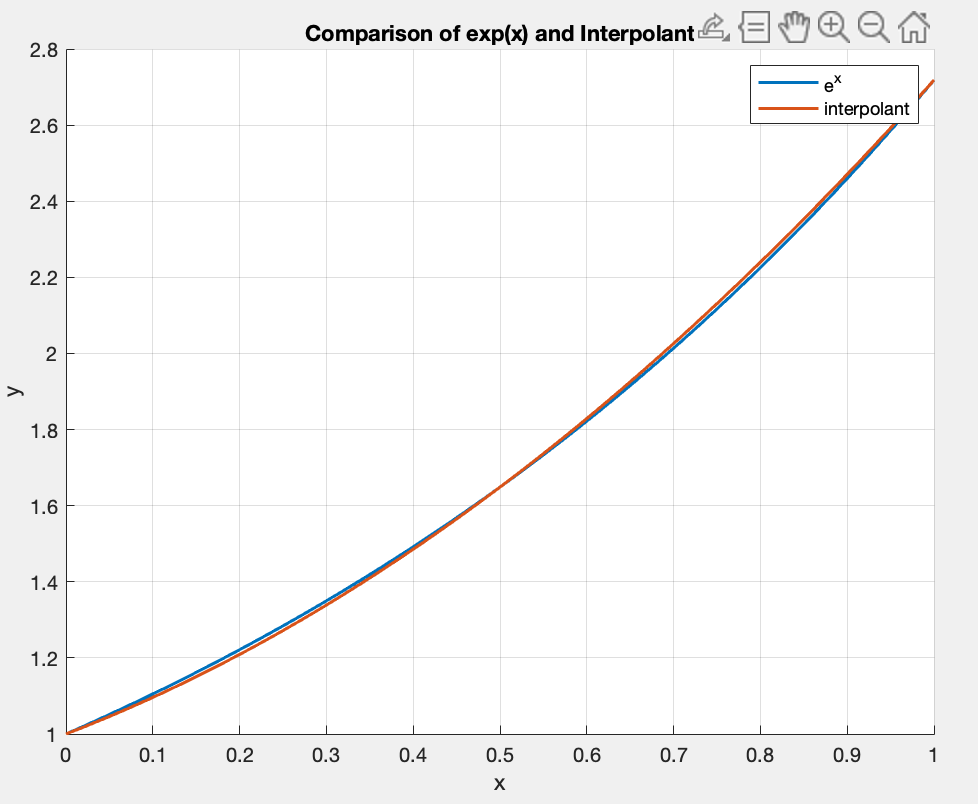
\includegraphics[width=0.6\textwidth]{q6c_plot.png} 
  \end{figure}
\end{solution}


\item Plot  the absolute error $|e^x - p_2(x)|$ on the interval using
logarithmic scale (the command {\tt semilogy}) and briefly compare
the error to the error bound you found in part (b).
\begin{solution}
  The following code was used to plot the absolute difference between the function $e^x$ 
  and the interpolant $p_2(x)$ and the error bound we found in  part (b).

  \begin{verbatim}
  a = 1;
  b = 2 * exp(1/2) - 2;
  c = 2 * exp(1) - 4 * exp(1/2) + 2;
  exponential = @(x) exp(x);
  interpolant = @(x) a + b .* x + c .* x .* (x - 1/2);
  
  abs_diff = @(x) abs(exp(x) - (a + b .* x + c .* x .* (x - 1/2)));

  x_values = linspace(0, 1, 100);

  y_values = abs_diff(x_values);

  current_error_bound = sqrt(3) * exp(1) / 216;
  error_bound_line = current_error_bound * ones(size(x_values));
  display(current_error_bound)


  hold on;
  semilogy(x_values, error_bound_line, 'LineWidth', 1.5);
  semilogy(x_values, y_values, 'LineWidth', 1.5);
  xlabel('x');
  ylabel('Absolute Difference');
  title('Absolute Difference with Logarithmic Scale');
  grid on;
  \end{verbatim}
  
  When plotted, we get the following plot,
\begin{figure}[H]
    \centering
    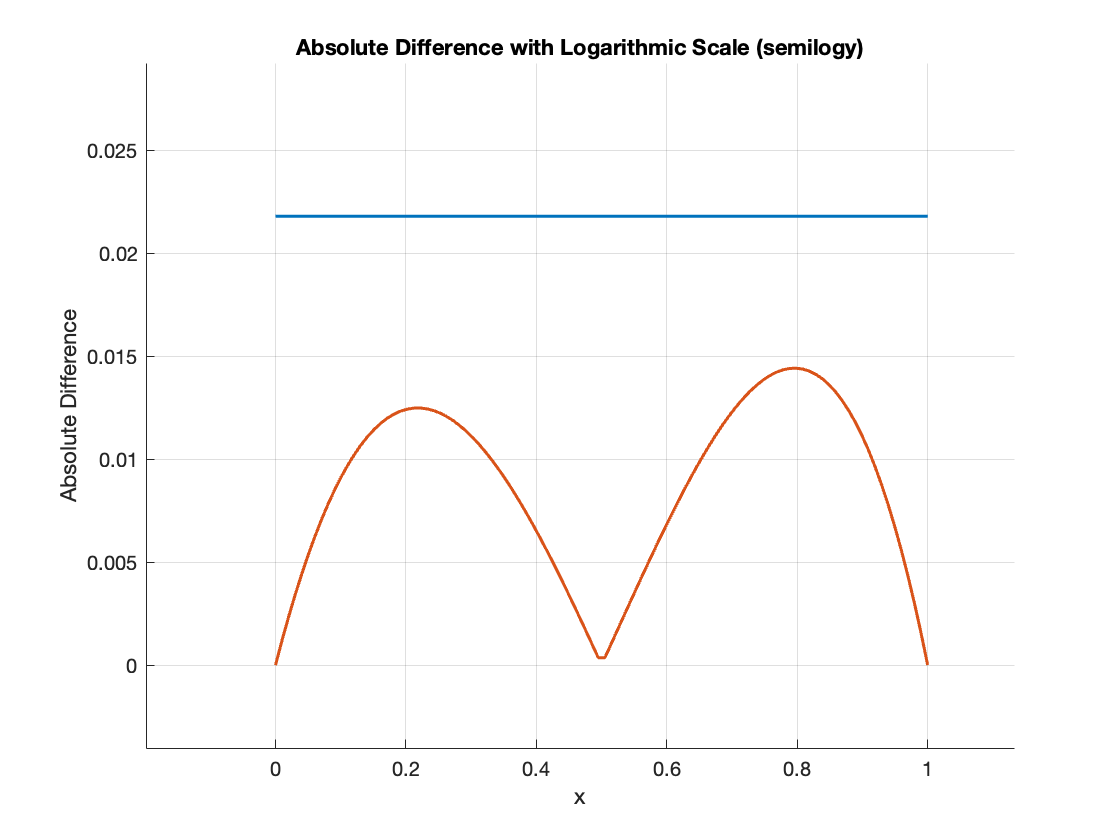
\includegraphics[width=0.6\textwidth]{q6d_plot.png} 
  \end{figure}
  We can see that the absolute error of the interpolant and the function is lower than the maximum bound that we have computed.

\end{solution}


\end{enumerate}

 \end{enumerate}

\end{document}
